\section{Soft constraint automata (2 pages)}

\paragraph{Constraints}
Consider a fixed rational component.
The relation between its ports is realized by satisfying certain constraints.
In addition to the previously defined set $P$ of port variables $p\in P$,
we let $M$ be a countably infinite set of memory cells, disjoint with $P$.
Memory cells can be intuitively understood as variable storage for components.
Then by $\underline{m}$ and $\underline{m}'$ we
denote\footnote{
	This notation is different than \cite{jongmans}, where $^\bullet m$ and $m^\bullet$ are used.
	This is to keep our syntax close in line with stream semantics.}
the variable for current value, and next value, respectively.
We let $\underline{M}=\{\underline{m}\mid m\in M\}$ and $\underline{M'}=\{\underline{m'}\mid m\in M\}$.
The constant symbol $*$ stands for no activity.
The symbol $f$, resp. $Q$, stands for a function, resp. predicate, with fixed arity $n$.

\begin{definition} A \textbf{term} $t$ is defined inductively as:
	$$ t \quad ::= \quad p \quad|
		\quad \underline{m} \quad|
		\quad \underline{m}' \quad|
		\quad f(t_1, ..., t_n) \quad|
		\quad * $$
	A \textbf{constraint} is a formula $\phi$ defined inductively as:
	$$ \phi \quad ::= \quad \bot \quad |
		\quad t_1 = t_2 \quad|
		\quad Q(t_1, ... , t_n) \quad|
		\quad \neg \phi \quad|
		\quad \exists p \phi \quad|
		\quad \phi_1 \land \phi_2 $$
\end{definition}

We use the following shorthand notations: $t_1 \not= t_2$ for $\neg (t_1=t_2)$,
and $\phi_1 \lor \phi_2$ for $\neg (\neg \phi_1 \land \neg\phi_2)$,
and $\forall p \phi$ for $\neg \exists p \neg\phi$.
We assume standard operator precedence.
Existential quantification only binds port variables,
and we consider constraints equal up to renaming of bound variables.
Let $V=P\cup\underline{M}\cup\underline{M'}$ be the set of all variables,
and let $V_{\phi}$ refer to the set of free variables occurring in $\phi$.

\paragraph{Model} Let $\mathcal{M}$ be a model containing the following data:
\begin{itemize}
	\item The set of data $D$;
	\item An interpretation $f^\mathcal{M} : D^n\rightarrow D$ for every function $f$ of arity $n$;
	\item An interpretation $Q^\mathcal{M}\subseteq D^n$ for every predicate $Q$ of arity $n$.
\end{itemize}
Nullary functions point to an element in $D$.
Recall that the alphabet $\Sigma$ contains data $D$ and $*$, and that $*\not\in D$.
We also call $\Sigma$ the set of observations.
Assume that we are given an assignment $\gamma:V\rightarrow\Sigma$ of variables to observations.
We define the observation of a term denoted $t^\mathcal{M}\in\Sigma$ such that:
$v^\mathcal{M}=\gamma(v)$ for all $v\in V$ and $*^\mathcal{M}=*$;
a function $f(t_1,...,t_n)^\mathcal{M}=f^\mathcal{M}(t_1^\mathcal{M},...,t_n^\mathcal{M})$ if
all $t_i^\mathcal{M}\in D$, and otherwise $f(t_1,...,t_n)^\mathcal{M}=*$.

\begin{definition}
	The \textbf{satisfaction relation} $\mathcal{M}, \gamma \models \phi$ is defined inductively as:
\begin{align*}
	\mathcal{M}, \gamma \models t_1=t_2 \quad &\Leftrightarrow \quad t_1^\mathcal{M}=t_2^\mathcal{M}; \\
	\mathcal{M}, \gamma \models Q(t_1,...,t_n) \quad &\Leftrightarrow \quad (t_1^\mathcal{M},...,t_n^\mathcal{M}) \in Q^\mathcal{M}; \\
	\mathcal{M}, \gamma \models \neg\phi \quad &\Leftrightarrow \quad \mathcal{M}, \gamma \not\models \phi ; \\
	\mathcal{M}, \gamma \models \exists p\phi \quad &\Leftrightarrow \quad \mathcal{M}, \gamma[p \mapsto x ] \models \phi \text{ for some }x \in \Sigma ; \\
	\mathcal{M}, \gamma \models \phi_1\land\phi_2 \quad &\Leftrightarrow \quad \mathcal{M}, \gamma \models \phi_1\text{ and }\mathcal{M}, \gamma \models \phi_2.
\end{align*}	
\end{definition}
Note that $\mathcal{M}, \gamma \not\models \bot$.
We define the assignment update $\gamma[x \mapsto m](x) = m$ and $\gamma[x \mapsto m](y) = \gamma(y)$ for $y\neq x$.

\paragraph{Solving} 
We fix some model $\mathcal{M}$.
The solutions of a constraint $\phi$ is the set of all assignments such that the constraint is satisfied,
$i.e.$ $\Gamma_{\phi} = \{ \gamma \mid \mathcal{M},\gamma \models \phi \}$.
We call an assignment $\gamma$ a solution for $\phi$ if $\gamma\in\Gamma_{\phi}$.

In the upcoming paragraph on operational semantics, we will see particular subsets of solutions.
Intuitively, an environment restricts the possible solutions by assigning values to ports.
The remaining solutions represent the allowed non-deterministic behavior of the component.


%We call $\Gamma_C:V_C \rightarrow D\cup\{\varnothing\}$ the assignment map defined on the set of variable $V_C$ of a component $C$. Given $v\in V_C$, $\Gamma_C(v) = d \in D$ if $v$ is defined, or $\Gamma_C(v) = \varnothing$ if v is not defined. We consider initially a map $\Gamma_C$ on which some variables already have a value assigned ($\Gamma_C(v) \not = \varnothing$).

%We say that a port $p$ fires whenever $p \not = *$. If a port $p$ fires and the port equates another port $q$, then both ports must synchronize and observe the same data. The corresponding formula is : $p=q \land p \not= *$. The symbol $*$ models the case where no data is observed at the port or in the memory cell. Existential quantifier is equivalent to hiding a port. Once hidden, it is no longer possible to synchronize on the port, and the variable can be eliminated by substitution. We allow user defined functions and relation in our language. Since a variable can be shared with the environment, we call $pending$ value the value set by the environment on a free variable.

%We say that a constraint is satisfiable if there is an assignment for all its free variables that makes the constraint true. Finding such an assignment follows two steps. Lets call $\Gamma:V \rightarrow D\cup\{*\}$ the assignment map from variable to data or special symbol *. For each constraints, we start with an assignment map $\Gamma$ empty, meaning that all variables maps to $*$. We first look at all free variables involved in the constraint and update the map $\Gamma$ according to their $pending$ value.

\paragraph{Preferences} 
We first consider preferences as a technique to steer particular behavior,
in the case that a constraint admits multiple remaining solutions.
Steering allows for greater expressiveness in the design of components.

We will consider a partial order among solutions,
such that the behavior of a component is fixed by its maximal solutions.
In case that no maximum solution exists,
it is still possible to have non-deterministic behavior.
We introduce \emph{constaint semirings} (abbreviated as c-semiring),
algebraic structures that induces a partial order.

%Intuitively, constraints serve as guards for transition in SCA. From one state, if multiple constraint are satisfiable, multiple transitions could be taken. Since we want to locally determine which transition to take, we introduce csemiring, an algebraic structure that induces an order on the transitions.

\begin{definition} A \textbf{c-semiring} structure $(E,+,\times,1,0)$ is a set $E$:
	\begin{itemize}
		\item Closed under binary operations $+,\times:E\times E\to E$ and unique $1,0\in E$;
		\item An idempotent commutative monoid $(E,+,0)$ with absorbing element 1;
		\item A commutative monoid $(E,\times,1)$ with absorbing element 0;
		\item Multiplication $(\times)$ distributes over addition $(+)$ from either sides.
	\end{itemize} 
	In other words, a commutative idempotent semiring with $e+1=1$.
\end{definition}

%Let $A \subseteq E$, we use the prefix notation $\sum(A)$ to describe the sum of all elements of A.

A c-semiring admits a partial order $\leq_{E}$ over elements in $E$, defined as the smallest relation satisfying: $ e+e' = e' \Leftrightarrow e \leq_{E} e' \text{ for all } e,e' \in E $.
Let the set $C$ comprise all constraints. Given a constraint $\phi\in C$ and an element $e\in E$, we call the pair $(\phi,e)$ a \emph{soft constraint}.

\begin{definition}
	A \textbf{soft constraint automaton} (SCA) is: 
	\begin{itemize}
		\item A set of states $Q$ and an initial state $q_0\in Q$;
		\item ${\rightarrow} \subseteq Q \times C \times E \times Q$ is a finite relation called transition relation. 
		%A transition is denoted by $\left\langle q_i, c, s, p_i \right\rangle \in \rightarrow$
	\end{itemize}
\end{definition}
A transition $(q,\phi,e,q') \in{\rightarrow}$ is denoted as $q \xrightarrow{\phi,e} q'$.

\paragraph{Operational semantics}
Let there be a soft constraint automaton. Given $q\in Q$, we define the set of solutions found on all outgoing transitions of state $q$.
$$\Gamma(q) = \{(\gamma,e,q')\mid \mathcal{M},\gamma\models\phi\text{ and }(q,\phi,e,q') \in{\rightarrow}\}$$

Let $\delta:P\to\Sigma$ be an assignment of port variables only,
and let $\Delta$ be a non-empty subset of the set $\{\delta\mid\delta:P\to\Sigma\}$ of all such assignments. We assume an arbitrary $\Delta$ is given by the environment. Intuitively, all singleton sets correspond to an environment that fixes all ports. At the other extreme, the set of all possible assignments imposes no restriction on ports whatsoever.

%As mentioned previously, we consider a subset of the solutions $\Gamma(q)$.
%We remark that the map $\gamma_*$ defined as $ \gamma_*(x) = 
%\begin{cases}
%	* &\quad\text{if x}\in P \\ 
%	\underline{x} &\quad\text{if x} \in M  
%\end{cases}$
% is always contained in $\Delta$. If $|\Delta|=1$, $\gamma_*$ is the only possible assignment. If $\Delta = \Gamma(q)$, the environment does not remove any possible assignment. Assuming a $\Delta \subseteq \Gamma(q)$ from the environment,

Similarly, let $\mu:\underline{M}\to\Sigma$ be an assignment of memory cells only. The initial assignment of memory cells is defined $\mu^I(\underline{m})=*$. Given a $\gamma:V\to\Sigma$, we can obtain the next assignment of memory cells by restricting its domain to $\underline{M'}$. More precisely, we define $\gamma':\underline{M}\to\Sigma$ to be $\gamma'(\underline{m})=\gamma(\underline{m'})$.

Recall $\delta:P\to\Sigma$. Let port equivalence be defined as $\gamma\equiv_P\delta$ if and only if $\gamma(p)=\delta(p)$ for all $p\in P$, and similarly, let memory equivalence be defined as $\mu\equiv_M\gamma$ if and only if $\mu(\underline{m})=\gamma(\underline{m})$ for all $m\in M$. We now define the set of \emph{environmental solutions} as:
$$\Gamma(q,\mu,\Delta) = \{(\gamma, e, q')\in\Gamma(q) \mid \mu\equiv_M\gamma\equiv_P\delta\text{ for some }\delta\in\Delta\}$$

We lift the partial order $\leq_E$ to environmental solutions, i.e. given $(\phi_1,e_1,q'_1)$ and $(\phi_2,e_2,q'_2)$ we define $(\phi_1,e_1,q'_1)\leq(\phi_2,e_2,q'_2)$ if and only if $e_1 \leq_E e_2$. The elements of the set of environmental solutions are now related by our lifted partial order. We take the maximal elements of the environmental solutions, which we call the \emph{maximal environmental solutions}, denoted as $\bigvee\!\Gamma(q,\mu,\Delta)$.

Operational semantics of our soft constraint automaton is given as follows:

\begin{itemize}
	\item A \emph{configuration} $(q,\mu)$ is a state $q\in Q$ and a memory assignment $\mu:\underline{M}\to\Sigma$;
	\item For each non-empty $\Delta\subseteq\{\delta\mid\delta:P\to\Sigma\}$ and for each $(\gamma,e,q')\in\Gamma(q,\mu,\Delta)$, we relate the configurations $(q,\mu)$ and $(q',\gamma')$;
	\item We have as initial configuration $(q_0,\mu^I)$.
\end{itemize}

%Since the sum $\Gamma_q$ is disjoint, we can define $p : \bigwedge\Delta \rightarrow Q$, a function that choose non deterministically a tuple from $\bigwedge\Delta$, and return the next state in $A$.

%We call $\Delta_{\psi} = \{ \delta \mid D,\delta \models \psi \}$ the partial map that models the environment assignment. Since the environment is represented by an irrational component, it is not possible to finitely represents the relation on its ports as a constraint. However, we know that $V_{\psi} \cap V_{\phi} \not = \emptyset$ since $\phi$ has some free variables. Thus, in each state we take 

%We define the semantic of soft constraint automata $\mathcal{A} = \left\langle Q, \rightarrow, C, \mathbb{S}, q_{0} \right\rangle$ as follows.
%At each state $q$, we take the set of constraint $\mathcal{C}_q = \{c \in C | \exists q'\in Q, q \xrightarrow{(c,e)} q' \in \mathcal{A}\}$. For each constraint $c\in \mathcal{C}_q$, 
%Given a sca $A = \left\langle Q, \rightarrow, C, \mathbb{S}, q_{0}, \right\rangle$, and a state $q\in Q$, the operational semantic of Soft Constraint Automata follows two steps : assignment and constraint solving. We denote $V_c$ the set of free variables involved in the constraint $c \in C$ The assignment step takes all variables involved in the constraints and assign values defined by the environment. Since variables refer to ports or current (or next value of memory cells), assigning a value means reading the value from a port. Since a port can have no data (*) or the variable no value assign, the second step invoke a constraint solver to find an assignment to satisfy the constraint.

%\paragraph*{LTS}

\begin{example}
	We present the example of a dancing flying drone, and we show the description of a non trivial behavior. The component has four ports: $p_{west}$, $p_{east}$, $p_{north}$ and $p_{south}$. Each port is constrained by a formula. We note $east$, $west$, $south$ and $north$ the name of the constraint respectively responsible to the observable behavior moving east, west, south or north. Certain actions are mutually exclusives : it is not possible to move east and west, or south and north at the same time. This composability relation appears in the formulation of the constraint. We define : 
	\begin{align*}
		& \text{west} := p_{west} \not = * \land p_{east} = * \\
		& \text{east} := p_{east} \not = * \land p_{west} = * \\
		& \text{north} := p_{north} \not = * \land p_{north} = * \\
		& \text{south} := p_{south} \not = * \land p_{south} = * 
	\end{align*}

	\begin{figure}[t]
	\centering
	\label{fig:Components}{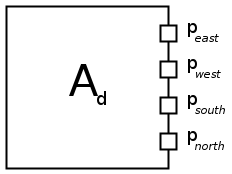
\includegraphics[scale=0.4]{pic/dancing_drone.png}}
	\qquad
	\caption{Soft constraint automata $A_d$ modeling the dance of the drone}
	\end{figure}
	
	\begin{figure}[H]
		\centering
		\resizebox{8cm}{!}{ \begin{tikzpicture}[>=latex,shorten >=1pt,node distance=3cm,on grid,auto, node/.style={circle,draw,minimum size=25pt}, ]

 \node[state] (qW) at (-40pt,0pt) {$q_W$};
 \node[state, right = of qW] (qN) {$q_N$};
 \node[state, below = of qW] (qS) {$q_S$};
 \node[state, right = of qS] (qE) {$q_E$};
 \draw[<-,text=white] (qW) -- node[] {} ++(0,1);
 \draw[->] (qN) to[out=160,in=20] node[above] {west , 2} (qW);
 \draw[->] (qS) to[out=-20,in=200] node[below] {east , 2} (qE);
 \draw[->] (qW) to[out=-110,in=110] node[left] {south , 2} (qS);
 \draw[->] (qE) to[out= 80,in=-80] node[right] {north, 2} (qN);
 \draw[->] (qN) to[out=20,in=-20,looseness=8] node[right, align=left] {east , 3\\south , 3 \\ north, 3} (qN);
 \draw[->] (qE) to[out=20,in=-20,looseness=8] node[right, align=left] {east , 3\\south , 3 \\ west, 3} (qE);
 \draw[->] (qW) to[out=160,in=-160,looseness=8] node[left, align=left] {west , 
 3 \\ east, 3 \\ north, 3} (qW);
 \draw[->] (qS) to[out=160,in=-160,looseness=8] node[left, align=left] {west , 3\\ south , 3 \\ north, 3} (qS);
 \end{tikzpicture}}
		\caption{Soft constraint automata $A_d$ modeling the dance of the drone}
		\label{moveSCA}
	\end{figure}

	The possible behaviors generated by the soft constraint automata of Fig. 2 correspond to the set of stream $\Sigma^{\omega}$, where a stream $\sigma \in \Sigma^{\omega}$ represents a trace of successive actions. The stream $(west,3)^{\omega} \in \Sigma^{\omega}$ represents the trace where the dancing drone always took the action $west$ in the initial state. As shown previously, the c-semiring value associated to the constraint induces a partial order on the set of behavior. In this example, if all constraints could be satisfied in each states, the best transition is the transition involving the soft constraint with the preference $2$. Thus, the best behavior is the stream $((south,2),(east,2),(north,2),(west,2))^{\omega}$, which corresponds to the dancing square of the drone.
	%$\{(west,3)^{\omega}, (east,3)^{\omega}, ((east,3),(south,2),(east,3)^{\omega}), ...\}$

%	This example present a protocol between three components : $east$,$west$ and $stay_{lon}$. Each components have one port, respectively named $p_{east}$, $p_west$ and $p_{stay_{lon}}$; and define a constraint $east := p_{east} \not = *$, $west := p_{west} \not = *$ and $stay_{lon} := p_{stay_{lon}} \not = *$. The constraint $idle := \neg east \land \neg west \land \neg stay_{lon}$ represents the assignment $\gamma_*$. We use the weighted c-semiring $(\mathbb{R}_+,+,\min,+\infty,0)$ and construct the following soft constraint automaton:
%	\begin{figure}[H]
%		\centering
%		\resizebox{8cm}{!}{ \begin{tikzpicture}[>=latex,shorten >=1pt,node distance=3cm,on grid,auto, node/.style={circle,draw,minimum size=25pt}, ]

 \node[state] (q0) at (-40pt,0pt) {$q_W$};
 \node[state, right = of q0] (q1) {$q_E$};
 \draw[<-,text=white] (q0) -- node[] {} ++(0,1);
 \draw[->] (q1) to[out=200,in=-20] node[below] {west , 5} (q0);
 \draw[->] (q0) to[out=20,in=160] node[above] {east , 5} (q1);
 \draw[->] (q1) to[out=20,in=-20,looseness=8] node[right, align=left] {east , 0\\stay$_{lon}$ , 5} (q1);
 \draw[->] (q0) to[out=160,in=-160,looseness=8] node[left, align=left] {west , 0\\ stay$_{lon}$ , 5} (q0);
 \end{tikzpicture}
}
%		\caption{Soft constraint automata for moving}
%		\label{moveSCA}
%	\end{figure}
\end{example}
\vfill